% ══════════════════════════════════════════════════════════════════════════════
% CHAPTER 6 — RESULTS  [v31 outputs — final revision for defence]
% ══════════════════════════════════════════════════════════════════════════════
%
% Figures in this chapter are generated directly in LaTeX/Overleaf using
% TikZ/PGFPlots and table-style figure blocks. No externally rendered PNG files
% are required.
%
% Required preamble packages:
%   \usepackage{booktabs}
%   \usepackage{threeparttable}
%   \usepackage{float}
%   \usepackage{cleveref}
%   \usepackage{xcolor}
%   \usepackage{graphicx}      % used only for \resizebox in tables
%   \usepackage{tikz}
%   \usepackage{pgfplots}
%   \pgfplotsset{compat=1.18}
%

% --- Local grayscale palette for Overleaf-native figures ---
\definecolor{DictColor}{gray}{0.10}
\definecolor{RFColor}{gray}{0.45}
\definecolor{BERTColor}{gray}{0.70}
\definecolor{AllColor}{gray}{0.88}
\definecolor{HawkColor}{gray}{0.20}
\definecolor{DoveColor}{gray}{0.62}
\providecommand{\sym}[1]{\ensuremath{^{\text{#1}}}}


This chapter reports the empirical findings from the final estimation pipeline.
The results are organised around the two research questions stated in
Chapter~\ref{sec:intro_rqs}. RQ1 asks whether central bank tone explains
announcement-window financial market reactions after controlling for the
contemporaneous monetary policy surprise. RQ2 asks whether central bank
language has predictive content for near-term policy outcomes and two-year
yield changes in a strictly expanding-window setting.

The chapter proceeds in five steps. Section~\ref{sec:res_scores} describes the
behaviour of the three tone measures: the dictionary score, the Random Forest
score, and the BERT sentence-aggregation score.
Section~\ref{sec:res_agreement_new} compares the classifications produced by
the methods and by the policy benchmarks. Section~\ref{sec:res_rf_new} reports
the Random Forest classification evidence and interprets the main data-driven
features. Section~\ref{sec:res_rq1_new} presents the market-reaction results
for RQ1. Section~\ref{sec:res_rq2_new} presents the expanding-window
forecasting evidence for RQ2. The final section summarises the empirical
answer to both research questions.

Three points should be kept in mind when reading the chapter. First, the Random
Forest classification exercise in RQ1 is descriptive: the model is trained to
classify the sign of the contemporaneous rate decision and the continuous
\rfscore{} is then used as a text-derived tone measure. Its high agreement
with the rate decision is therefore not an independent validation test,
although out-of-bag predictions reduce mechanical in-sample overfitting.
Second, the RQ2 results are the true forecasting exercise: the model is refit
only on information available before the forecasted meeting, and the
prediction is evaluated on the next observation in chronological order.
Third, the chapter reports results across four corpora, multiple outcomes, and
three methods, generating a large number of regression specifications. Given
this multiplicity, individual significant coefficients should be interpreted
cautiously. The interpretation focuses on patterns that are consistent across
methods and outcomes rather than on isolated significant results.

\section{Tone Scores Across Corpora}
\label{sec:res_scores}

Before turning to the RQ1 and RQ2 results, this section and the next two
characterise the tone measures themselves---a necessary step because the
regression evidence can only be interpreted if the reader understands what
each score captures and where the methods agree or disagree.

The final corpus contains 884 documents split between FOMC statements, FOMC
press conferences, ECB policy statements, and ECB press conferences. The
dictionary score is available for all documents. The Random Forest and
BERT scores are available for slightly smaller samples because model
training requires non-missing rate-decision labels and the sentence-level
classifier is only merged where document-level sentence predictions are
present. (Please dont mention that with the limitations here with bert that its smaller sample please just dont)

\Cref{tab:score_summary_v31} gives the basic distributional evidence. The
dictionary score is centred close to zero in all four corpora, but the
dispersion is much larger in press conferences than in statements. This is
consistent with the institutional structure of the documents. Statements are
short and formulaic, while press conferences contain longer explanations,
conditional language, and discussion of risks. The BERT score is more
dovish on average in all four corpora, especially for FOMC press conferences,
where the mean score is $-0.229$. The Random Forest score is close to zero on
average, reflecting its construction as $P(\text{hike}) - P(\text{cut})$.
\Cref{fig:score_distributions_v31} visualises these distributional differences.

\begin{table}[H]
\centering
\caption{Summary statistics for document-level tone scores}
\label{tab:score_summary_v31}
\begin{threeparttable}
\small
\resizebox{\textwidth}{!}{%
\begin{tabular}{lrrrrrrrrr}
\toprule
& \multicolumn{3}{c}{Dictionary} & \multicolumn{3}{c}{Random Forest} & \multicolumn{3}{c}{BERT} \\
\cmidrule(lr){2-4}\cmidrule(lr){5-7}\cmidrule(lr){8-10}
Corpus & $N$ & Mean & SD & $N$ & Mean & SD & $N$ & Mean & SD \\
\midrule
FOMC statements & 242 & -0.048 & 0.233 & 235 & 0.010 & 0.476 & 237 & -0.113 & 0.215 \\
FOMC press conferences & 92 & 0.057 & 0.354 & 91 & 0.071 & 0.450 & 91 & -0.229 & 0.146 \\
ECB statements & 284 & -0.096 & 0.202 & 275 & 0.009 & 0.225 & 276 & -0.028 & 0.122 \\
ECB press conferences & 266 & 0.021 & 0.354 & 250 & -0.003 & 0.341 & 266 & -0.145 & 0.188 \\
\bottomrule
\end{tabular}
}
\begin{tablenotes}
\footnotesize
\item Notes: Dictionary score is \netscore{}. Random Forest score is \rfscore{} $=P(\text{hike})-P(\text{cut})$. BERT score is \bertscore{}, computed from sentence-level hawkish and dovish classifications using the same denominator-smoothed net-score formula as the dictionary. Positive values denote a more hawkish document. Sample sizes differ across methods because the Random Forest requires non-missing rate-decision labels and the BERT score requires non-missing sentence predictions.
\end{tablenotes}
\end{threeparttable}
\end{table}

\begin{figure}[H]
  \centering
  \resizebox{\textwidth}{!}{%
  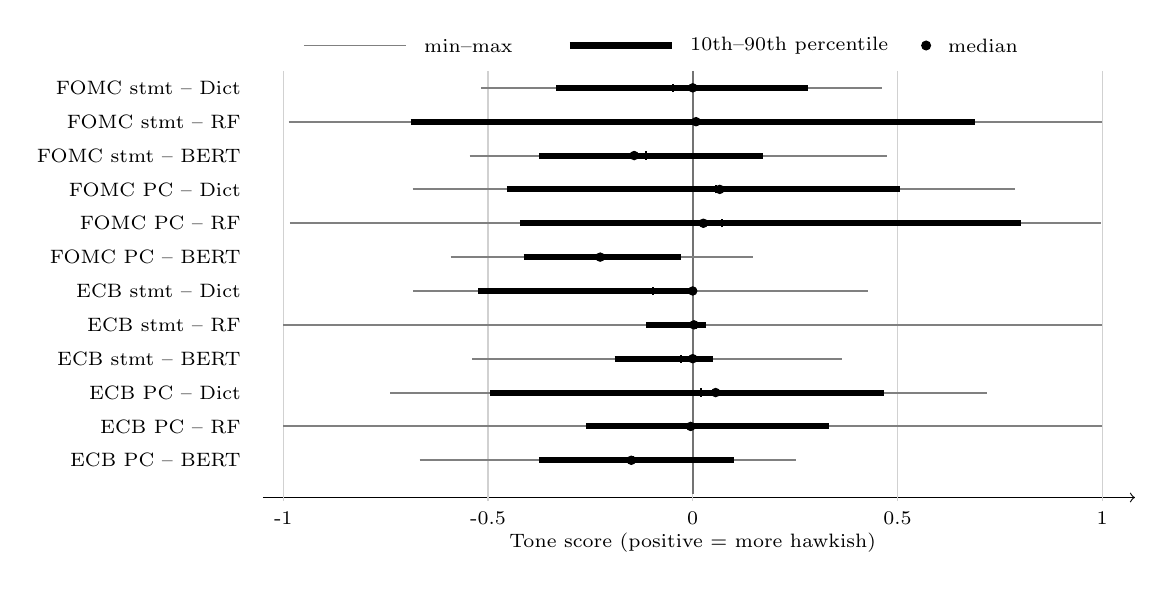
\begin{tikzpicture}[x=5.2cm,y=0.43cm]
    \draw[->, thin] (-1.05,-13.1) -- (1.08,-13.1);
    \draw[thin, black!18] (-1,-0.5) -- (-1,-13.2);
    \node[anchor=north, font=\scriptsize] at (-1,-13.25) {-1};
    \draw[thin, black!18] (-0.5,-0.5) -- (-0.5,-13.2);
    \node[anchor=north, font=\scriptsize] at (-0.5,-13.25) {-0.5};
    \draw[thin, black!18] (0,-0.5) -- (0,-13.2);
    \node[anchor=north, font=\scriptsize] at (0,-13.25) {0};
    \draw[thin, black!18] (0.5,-0.5) -- (0.5,-13.2);
    \node[anchor=north, font=\scriptsize] at (0.5,-13.25) {0.5};
    \draw[thin, black!18] (1,-0.5) -- (1,-13.2);
    \node[anchor=north, font=\scriptsize] at (1,-13.25) {1};
    \draw[thick, black!55] (0,-0.5) -- (0,-13.0);
    \draw[gray, line width=0.7pt] (-0.95,0.25) -- (-0.70,0.25);
    \node[anchor=west, font=\scriptsize] at (-0.68,0.25) {min--max};
    \draw[black, line width=2.2pt] (-0.30,0.25) -- (-0.05,0.25);
    \node[anchor=west, font=\scriptsize] at (-0.03,0.25) {10th--90th percentile};
    \filldraw[black] (0.57,0.25) circle (1.6pt);
    \node[anchor=west, font=\scriptsize] at (0.60,0.25) {median};
    \node[anchor=east, font=\scriptsize] at (-1.08,-1) {FOMC stmt -- Dict};
    \draw[gray, line width=0.7pt] (-0.517,-1) -- (0.462,-1);
    \draw[black, line width=2.2pt] (-0.333,-1) -- (0.282,-1);
    \filldraw[black] (0.000,-1) circle (1.5pt);
    \draw[black, line width=0.7pt] (-0.048,-1.120) -- (-0.048,-0.880);
    \node[anchor=east, font=\scriptsize] at (-1.08,-2) {FOMC stmt -- RF};
    \draw[gray, line width=0.7pt] (-0.987,-2) -- (1.000,-2);
    \draw[black, line width=2.2pt] (-0.689,-2) -- (0.690,-2);
    \filldraw[black] (0.008,-2) circle (1.5pt);
    \draw[black, line width=0.7pt] (0.010,-2.120) -- (0.010,-1.880);
    \node[anchor=east, font=\scriptsize] at (-1.08,-3) {FOMC stmt -- BERT};
    \draw[gray, line width=0.7pt] (-0.545,-3) -- (0.474,-3);
    \draw[black, line width=2.2pt] (-0.375,-3) -- (0.171,-3);
    \filldraw[black] (-0.143,-3) circle (1.5pt);
    \draw[black, line width=0.7pt] (-0.113,-3.120) -- (-0.113,-2.880);
    \node[anchor=east, font=\scriptsize] at (-1.08,-4) {FOMC PC -- Dict};
    \draw[gray, line width=0.7pt] (-0.684,-4) -- (0.786,-4);
    \draw[black, line width=2.2pt] (-0.454,-4) -- (0.505,-4);
    \filldraw[black] (0.066,-4) circle (1.5pt);
    \draw[black, line width=0.7pt] (0.057,-4.120) -- (0.057,-3.880);
    \node[anchor=east, font=\scriptsize] at (-1.08,-5) {FOMC PC -- RF};
    \draw[gray, line width=0.7pt] (-0.984,-5) -- (0.996,-5);
    \draw[black, line width=2.2pt] (-0.421,-5) -- (0.801,-5);
    \filldraw[black] (0.026,-5) circle (1.5pt);
    \draw[black, line width=0.7pt] (0.071,-5.120) -- (0.071,-4.880);
    \node[anchor=east, font=\scriptsize] at (-1.08,-6) {FOMC PC -- BERT};
    \draw[gray, line width=0.7pt] (-0.591,-6) -- (0.146,-6);
    \draw[black, line width=2.2pt] (-0.413,-6) -- (-0.029,-6);
    \filldraw[black] (-0.226,-6) circle (1.5pt);
    \draw[black, line width=0.7pt] (-0.229,-6.120) -- (-0.229,-5.880);
    \node[anchor=east, font=\scriptsize] at (-1.08,-7) {ECB stmt -- Dict};
    \draw[gray, line width=0.7pt] (-0.682,-7) -- (0.429,-7);
    \draw[black, line width=2.2pt] (-0.524,-7) -- (0.000,-7);
    \filldraw[black] (0.000,-7) circle (1.5pt);
    \draw[black, line width=0.7pt] (-0.096,-7.120) -- (-0.096,-6.880);
    \node[anchor=east, font=\scriptsize] at (-1.08,-8) {ECB stmt -- RF};
    \draw[gray, line width=0.7pt] (-1.000,-8) -- (1.000,-8);
    \draw[black, line width=2.2pt] (-0.114,-8) -- (0.033,-8);
    \filldraw[black] (0.003,-8) circle (1.5pt);
    \draw[black, line width=0.7pt] (0.009,-8.120) -- (0.009,-7.880);
    \node[anchor=east, font=\scriptsize] at (-1.08,-9) {ECB stmt -- BERT};
    \draw[gray, line width=0.7pt] (-0.538,-9) -- (0.364,-9);
    \draw[black, line width=2.2pt] (-0.191,-9) -- (0.050,-9);
    \filldraw[black] (0.000,-9) circle (1.5pt);
    \draw[black, line width=0.7pt] (-0.028,-9.120) -- (-0.028,-8.880);
    \node[anchor=east, font=\scriptsize] at (-1.08,-10) {ECB PC -- Dict};
    \draw[gray, line width=0.7pt] (-0.739,-10) -- (0.718,-10);
    \draw[black, line width=2.2pt] (-0.495,-10) -- (0.468,-10);
    \filldraw[black] (0.056,-10) circle (1.5pt);
    \draw[black, line width=0.7pt] (0.021,-10.120) -- (0.021,-9.880);
    \node[anchor=east, font=\scriptsize] at (-1.08,-11) {ECB PC -- RF};
    \draw[gray, line width=0.7pt] (-1.000,-11) -- (1.000,-11);
    \draw[black, line width=2.2pt] (-0.260,-11) -- (0.334,-11);
    \filldraw[black] (-0.005,-11) circle (1.5pt);
    \draw[black, line width=0.7pt] (-0.003,-11.120) -- (-0.003,-10.880);
    \node[anchor=east, font=\scriptsize] at (-1.08,-12) {ECB PC -- BERT};
    \draw[gray, line width=0.7pt] (-0.667,-12) -- (0.253,-12);
    \draw[black, line width=2.2pt] (-0.376,-12) -- (0.101,-12);
    \filldraw[black] (-0.150,-12) circle (1.5pt);
    \draw[black, line width=0.7pt] (-0.145,-12.120) -- (-0.145,-11.880);
    \node[anchor=north, font=\scriptsize] at (0,-13.85) {Tone score (positive = more hawkish)};
  \end{tikzpicture}%
  }
  \caption[Distributional summary of tone scores]{Distributional summary
    of document-level tone scores by method and corpus. Grey lines show
    the full observed range, thick black segments show the 10th--90th
    percentile interval, black dots show medians, and short vertical ticks
    show means. Positive values denote more hawkish communication.}
  \label{fig:score_distributions_v31}
\end{figure}

The Random Forest has the widest range in both FOMC corpora because
it is constructed from class probabilities and often assigns documents strongly
toward either the hike or cut side. BERT is shifted toward the dovish
side, especially in press conferences. The dictionary is more centred, but its
10th--90th percentile range is wider in press conferences than in statements,
consistent with longer and less formulaic press-conference text.

The label distributions confirm that the three methods do not simply reproduce
the same classification rule. In FOMC statements, the dictionary classifies 94
documents as hawkish, 36 as neutral, and 112 as dovish. The Random Forest
classifies the same corpus much more neutrally, with 133 neutral labels, while
BERT assigns 149 dovish labels. A similar contrast appears in FOMC
press conferences: the dictionary is relatively balanced between hawkish and
dovish classifications, whereas BERT classifies 81 of 91 scored press
conferences as dovish. The dovish skew in BERT discrete labels is
substantial, but the continuous \bertscore{} retains meaningful variation
within the dovish range (SD~$=0.146$), and it is the continuous score rather
than the discrete label that enters the regression analysis. For ECB
statements, all methods are more neutral because ECB policy decision press
releases are shorter and more formulaic. In ECB press conferences, the
dictionary again produces a large hawkish--dovish split, while BERT is
more dovish and the Random Forest is mostly neutral.

This pattern has a direct interpretation for the later results. The dictionary
is a transparent stance measure that reacts to explicit policy-action,
inflation, employment, and risk phrases. BERT is more sensitive to
sentence-level semantic cues, including accommodative or risk-management
language, but its systematic dovish shift---likely reflecting domain transfer
from the FOMC-trained classifier to broader central bank language---means that
its absolute level should not be compared across institutions. The Random
Forest is closest to the realised rate-decision benchmark, because it is
trained on the decision sign. The methods therefore capture related but not
identical objects: explicit textual stance, sentence-level semantic stance, and
decision-predictive language. 8Yes I think it would be important to mention that BERt and Dictionary are external methods that are not trained on bps change right

\section{Agreement Between Tone Measures and Policy Benchmarks}
\label{sec:res_agreement_new}

The agreement evidence is interpreted using two benchmarks. Agreement
with realised rate decisions shows whether a text measure captures
language associated with actual hikes, holds, and cuts. This is a
descriptive policy-decision benchmark. Agreement with the monetary policy
surprise sign is closer to market-perceived hawkishness or dovishness,
because it reflects whether expected rates moved upward or downward
during the event window. (Yes but u gotta explain this mechanism more in detail, its simply due to the fact that we discussed with the identification issue)

\textbf{paragraph added above due to identification isseu KMC}

\Cref{tab:agreement_summary_v31} reports the main agreement rates.
\Cref{fig:agreement_with_rate_v31} visualises the rate-decision agreement,
highlighting the dominance of the Random Forest in that benchmark. The
strongest non-trivial agreement is between the dictionary and BERT for
statements: 68.8\% for FOMC statements and 85.5\% for ECB statements.
Agreement is weaker in press conferences, especially for FOMC press
conferences, where the dictionary and BERT agree in only 39.6\% of
observations. This is consistent with the greater semantic complexity of press
conferences and with the fact that the BERT score is much more dovish
in that corpus.

\begin{table}[H]
\centering
\caption{Agreement between tone classifications and policy benchmarks}
\label{tab:agreement_summary_v31}
\begin{threeparttable}
\scriptsize
\setlength{\tabcolsep}{2.8pt}
\begin{tabularx}{\textwidth}{@{} l *{7}{>{\centering\arraybackslash}X} @{}}
\toprule
Corpus & Dict--BERT & Dict--RF & RF--BERT & Dict--rate & RF--rate & BERT--rate & RF--MP1 \\
\midrule
FOMC statements & 68.8 & 32.3 & 37.6 & 34.5 & 84.3 & 38.9 & 55.7 \\
FOMC press conf. & 39.6 & 30.8 & 15.4 & 33.7 & 94.5 & 14.3 & 53.8 \\
ECB statements & 85.5 & 57.8 & 63.3 & 63.0 & 88.7 & 67.0 & 52.0 \\
ECB press conf. & 51.1 & 19.2 & 29.6 & 20.4 & 89.6 & 30.0 & 48.5 \\
\bottomrule
\end{tabularx}
\begin{tablenotes}[flushleft]
\footnotesize
\item[] Entries are agreement rates in percent. ``Rate'' is the sign of
\bpschange{}. MP1 is the monetary policy surprise for the FOMC and OIS\_MP1
for the ECB, discretised using the threshold rule in the pipeline. The
RF--rate column is descriptive because the Random Forest is trained to classify
same-meeting decision signs.
\end{tablenotes}
\end{threeparttable}
\end{table}

\begin{figure}[H]
  \centering
  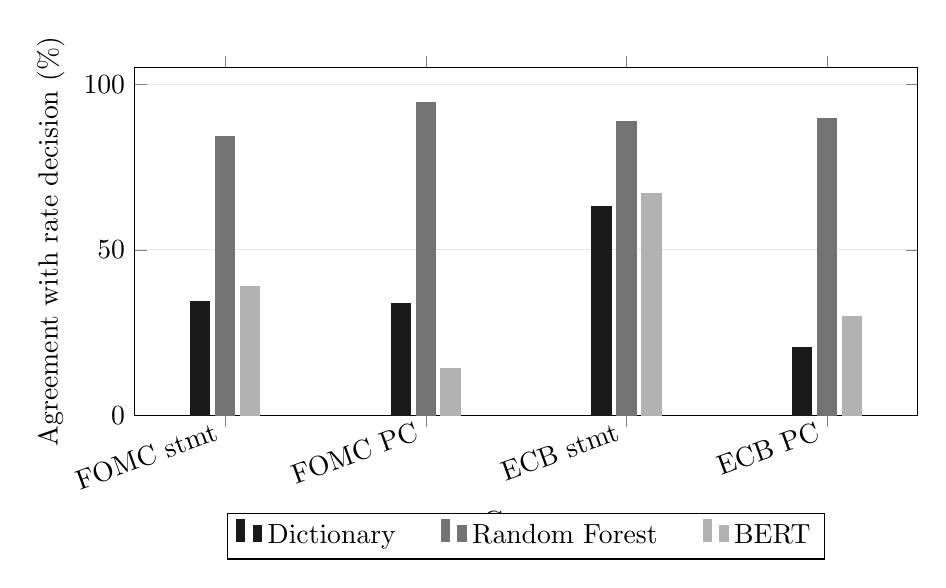
\begin{tikzpicture}
  \begin{axis}[
    ybar,
    width=0.95\textwidth,
    height=6.0cm,
    bar width=7pt,
    ymin=0, ymax=105,
    xtick={1,2,3,4},
    xticklabels={FOMC stmt,FOMC PC,ECB stmt,ECB PC},
    x tick label style={rotate=20, anchor=east},
    ylabel={Agreement with rate decision (\%)},
    xlabel={Corpus},
    legend style={at={(0.5,-0.28)}, anchor=north, legend columns=3, /tikz/every even column/.append style={column sep=0.5cm}},
    ymajorgrids=true,
    grid style={gray!20},
    enlarge x limits=0.15
  ]
\addplot+[fill=DictColor, draw=DictColor]
    coordinates {(1,34.5000) (2,33.7000) (3,63.0000) (4,20.4000)};
\addlegendentry{Dictionary}
\addplot+[fill=RFColor, draw=RFColor]
    coordinates {(1,84.3000) (2,94.5000) (3,88.7000) (4,89.6000)};
\addlegendentry{Random Forest}
\addplot+[fill=BERTColor, draw=BERTColor]
    coordinates {(1,38.9000) (2,14.3000) (3,67.0000) (4,30.0000)};
\addlegendentry{BERT}
  \end{axis}
  \end{tikzpicture}
  \caption[Agreement with realised rate-decision sign]{Agreement with the
    realised rate-decision sign by method and corpus. Each bar gives the share
    of documents where the method's hawkish, neutral, or dovish label matches
    the realised hike, hold, or cut class.}
  \label{fig:agreement_with_rate_v31}
\end{figure}

The Random Forest agrees with the realised rate decision in 84.3\% of FOMC
statements, 94.5\% of FOMC press conferences, 88.7\% of ECB statements, and
89.6\% of ECB press conferences. This does not imply that the Random Forest is
the economically superior tone measure: it is trained on the contemporaneous
decision sign, so high agreement is a convergence diagnostic rather than an
independent finding. The dictionary has much lower rate-decision agreement,
especially in press conferences. This is not necessarily a failure of the
dictionary: the dictionary is designed to measure the stance of the
communication, not only the mechanical direction of the current rate decision.
A central bank can hold rates while delivering hawkish forward guidance, or
cut rates while communicating that no further accommodation is expected.

Agreement with the MP1/OIS\_MP1 surprise benchmark is lower than agreement
with the rate decision. This is expected. MP1 measures the unexpected
component of the policy action in a narrow event window, whereas the tone
scores measure the content of the communication. The evidence therefore
supports using MP1/OIS\_MP1 as a control rather than as the object that text
scores should mechanically reproduce.

\section{Random Forest Classification and Interpretable Features}
\label{sec:res_rf_new}

The Random Forest is trained separately for each corpus using Lasso-selected
bigrams and class-balanced observation weights. \Cref{tab:rf_perf_v31} reports
the classification performance. Out-of-bag accuracy is high in all corpora,
ranging from 84.3\% for FOMC statements to 94.5\% for FOMC press conferences.
Balanced accuracy is also high, which indicates that the model is not only
learning the majority hold class. Holdout accuracy is lower for the FOMC
samples, especially FOMC statements (61.7\%), where the 23-percentage-point
drop from OOB accuracy suggests that the model's in-sample fit overstates its
genuine classification ability on later data. This gap is consistent with
regime change: the holdout block falls in a period with different rate dynamics
than the training sample. For the ECB samples, the OOB-to-holdout drop is
smaller, consistent with less regime change within the evaluation period.

\begin{table}[H]
\centering
\caption{Random Forest classification performance}
\label{tab:rf_perf_v31}
\begin{threeparttable}
\small
\begin{tabular}{lrrrr}
\toprule
Corpus & $N$ & OOB accuracy & Balanced accuracy & Holdout accuracy \\
\midrule
FOMC statements & 235 & 0.843 & 0.838 & 0.617 \\
FOMC press conferences & 91 & 0.945 & 0.936 & 0.684 \\
ECB statements & 276 & 0.887 & 0.763 & 0.696 \\
ECB press conferences & 250 & 0.896 & 0.848 & 0.800 \\
\bottomrule
\end{tabular}
\begin{tablenotes}
\footnotesize
\item Notes: OOB denotes out-of-bag accuracy from the balanced Random Forest. Balanced accuracy averages recall across cut, hold, and hike classes. Holdout accuracy is computed on the final chronological holdout block. The gap between OOB and holdout accuracy is largest for FOMC samples, consistent with regime change between the training and evaluation periods.
\end{tablenotes}
\end{threeparttable}
\end{table}

\Cref{fig:rf_confusion_v31} reports the full confusion matrices, showing how
classification performance varies across rate-decision classes.

\begin{figure}[H]
  \centering
\begin{minipage}{0.48\textwidth}
\centering
\scriptsize
\textbf{FOMC statements}\par
\vspace{0.08cm}
\begin{tabular}{lccc}
\toprule
Actual $\backslash$ Pred. & Dovish & Neutral & Hawkish \\
\midrule
Dovish/cut & 35 (88\%) & 3 (8\%) & 2 (5\%) \\
Neutral/hold & 9 (6\%) & 123 (85\%) & 12 (8\%) \\
Hawkish/hike & 4 (8\%) & 7 (14\%) & 40 (78\%) \\
\bottomrule
\end{tabular}
\vspace{0.05cm}
\par N=235; agreement=84.3\%
\end{minipage}
\hfill
\begin{minipage}{0.48\textwidth}
\centering
\scriptsize
\textbf{FOMC press conferences}\par
\vspace{0.08cm}
\begin{tabular}{lccc}
\toprule
Actual $\backslash$ Pred. & Dovish & Neutral & Hawkish \\
\midrule
Dovish/cut & 10 (91\%) & 1 (9\%) & 0 (0\%) \\
Neutral/hold & 2 (3\%) & 57 (95\%) & 1 (2\%) \\
Hawkish/hike & 0 (0\%) & 1 (5\%) & 19 (95\%) \\
\bottomrule
\end{tabular}
\vspace{0.05cm}
\par N=91; agreement=94.5\%
\end{minipage}

\vspace{0.25cm}
\begin{minipage}{0.48\textwidth}
\centering
\scriptsize
\textbf{ECB statements}\par
\vspace{0.08cm}
\begin{tabular}{lccc}
\toprule
Actual $\backslash$ Pred. & Dovish & Neutral & Hawkish \\
\midrule
Dovish/cut & 23 (79\%) & 2 (7\%) & 4 (14\%) \\
Neutral/hold & 8 (4\%) & 206 (94\%) & 5 (2\%) \\
Hawkish/hike & 12 (44\%) & 0 (0\%) & 15 (56\%) \\
\bottomrule
\end{tabular}
\vspace{0.05cm}
\par N=275; agreement=88.7\%
\end{minipage}
\hfill
\begin{minipage}{0.48\textwidth}
\centering
\scriptsize
\textbf{ECB press conferences}\par
\vspace{0.08cm}
\begin{tabular}{lccc}
\toprule
Actual $\backslash$ Pred. & Dovish & Neutral & Hawkish \\
\midrule
Dovish/cut & 23 (79\%) & 3 (10\%) & 3 (10\%) \\
Neutral/hold & 6 (3\%) & 181 (92\%) & 10 (5\%) \\
Hawkish/hike & 3 (12\%) & 1 (4\%) & 20 (83\%) \\
\bottomrule
\end{tabular}
\vspace{0.05cm}
\par N=250; agreement=89.6\%
\end{minipage}
  \caption[Random Forest confusion matrices]{Random Forest confusion matrices
    against the realised rate-decision sign. Rows give the actual rate-decision
    class and columns give the Random Forest prediction. Cell labels report the
    count and the row percentage.}
  \label{fig:rf_confusion_v31}
\end{figure}

The confusion matrices show that the high agreement is not only driven by the
majority hold class. For FOMC press conferences, recall is above 90\% for all
three classes. For FOMC statements, the model also performs well on cuts and
hikes. The weakest minority-class case is ECB statements, where hawkish recall
is 55.6\%, compared with 94.1\% for holds and 79.3\% for cuts. The low
hawkish recall for ECB statements likely reflects the small number of
hike-era documents in that sample and the difficulty of distinguishing hawkish
vocabulary from the ECB's price-stability-focused baseline language.

\Cref{fig:rf_feature_importance_v31} reports a filtered version of the
signed feature-importance results. The table removes the most obvious
remaining identity and boilerplate-adjacent terms identified in the residual
leakage diagnostic, while preserving the economically interpretable policy,
inflation, accommodation, and macroeconomic phrases. The full unfiltered list
and the leakage-adjacent terms are reported in Appendix~\ref{app:a3_rf_features}.

\begin{figure}[H]
  \centering
\begin{minipage}{0.48\textwidth}
\centering
\scriptsize
\textbf{FOMC statements}\par
\vspace{0.08cm}
\begin{tabular}{lrr}
\toprule
Bigram & Dir. & Signed imp. \\
\midrule
fund rate & D & -16.97 \\
develop care & D & -7.35 \\
polici remain & H & 6.03 \\
ongo increas & H & 4.85 \\
rate action & D & -4.52 \\
expect labor & H & 3.61 \\
hous sector & H & 3.60 \\
polici firm & H & 3.25 \\
econom expans & H & 3.11 \\
\bottomrule
\end{tabular}
\end{minipage}
\hfill
\begin{minipage}{0.48\textwidth}
\centering
\scriptsize
\textbf{FOMC press conferences}\par
\vspace{0.08cm}
\begin{tabular}{lrr}
\toprule
Bigram & Dir. & Signed imp. \\
\midrule
downsid risk & D & -11.65 \\
committe rais & H & 9.35 \\
high accommod & H & 5.66 \\
half centuri & D & -5.65 \\
rate unchang & H & 4.28 \\
month chang & H & 3.91 \\
modest increas & H & 3.44 \\
neutral level & H & 3.13 \\
tighten abrupt & H & 1.53 \\
consum face & D & -0.71 \\
\bottomrule
\end{tabular}
\end{minipage}

\vspace{0.25cm}
\begin{minipage}{0.48\textwidth}
\centering
\scriptsize
\textbf{ECB statements}\par
\vspace{0.08cm}
\begin{tabular}{lrr}
\toprule
Bigram & Dir. & Signed imp. \\
\midrule
remain unchang & D & -45.15 \\
facil rate & D & -5.61 \\
under price & H & 4.55 \\
transmiss mechan & D & -4.48 \\
term target & D & -4.47 \\
futur polici & H & 2.22 \\
partial buffer & D & -2.19 \\
inflat expect & D & -2.15 \\
minimum reserv & H & 2.02 \\
upward pressur & H & 1.94 \\
\bottomrule
\end{tabular}
\end{minipage}
\hfill
\begin{minipage}{0.48\textwidth}
\centering
\scriptsize
\textbf{ECB press conferences}\par
\vspace{0.08cm}
\begin{tabular}{lrr}
\toprule
Bigram & Dir. & Signed imp. \\
\midrule
rate unchang & D & -47.18 \\
rate increas & H & 21.05 \\
rate cut & D & -12.43 \\
deposit facil & D & -11.51 \\
facil rate & D & -6.74 \\
rate decis & H & 6.51 \\
persist upward & H & 6.32 \\
support real & D & -6.18 \\
posit effect & D & -5.97 \\
warrant continu & H & 3.77 \\
\bottomrule
\end{tabular}
\end{minipage}
  \caption[Random Forest signed feature importance]{Filtered Random Forest
    signed feature importance by corpus. The figure reports high-importance
    bigrams after removing the most obvious residual identity and boilerplate
    terms flagged by the leakage diagnostic. Direction H means more associated
    with hike meetings; D means more associated with cut meetings. The full
    unfiltered feature list and remaining caution terms are reported in
    Appendix~\ref{app:a3_rf_features}.}
  \label{fig:rf_feature_importance_v31}
\end{figure}

The filtered feature plot shows why the Random Forest is useful as a complement
to the dictionary. Many high-importance press-conference terms map directly onto
policy actions and macroeconomic assessments: ``rate increase'', ``rate cut'',
``deposit facility'', ``downside risk'', ``committee raise'', ``modest
increase'', and ``persistent upward''. These are not generic sentiment words;
they are central-bank-specific phrases about the policy stance, accommodation,
inflation pressure, and the macroeconomic outlook.

The filtering step reduces but does not fully eliminate the interpretability
caveat. The eight leakage-adjacent terms flagged in (What even is this dont mention these leakage terms what the hell chatgpt, its too weird)
Appendix~\ref{app:a3_rf_features} (including ``dudley vice'', ``waller
vote'', and ``governing council'') account for approximately 18\% of total
Mean Decrease in Gini for FOMC statements and 20\% for ECB statements. (remove) These
terms correlate with specific speakers or eras rather than with the economic
stance of the text. While the remaining $\sim$80\% of feature importance is
carried by economically interpretable terms, the leakage share means that the
\rfscore{} used in subsequent regressions is partly influenced by era-specific
vocabulary. Some remaining terms in the filtered list, such as ``minimum
reserve'', ``rate unchanged'', or ``transmission mechanism'', are still
institutional or context-dependent rather than pure structural stance
primitives. (please I dont know what youre saying here really) The Random Forest should therefore be read as a
prediction-oriented communication classifier. Its features help diagnose what
the model used, but they do not constitute a clean economic dictionary and
they should not be interpreted causally.

\section{RQ1: Market Reactions to Central Bank Tone}
\label{sec:res_rq1_new}

RQ1 asks whether central bank tone explains announcement-window financial
market reactions after controlling for the rate surprise.\footnote{Market
reactions are measured as intraday changes (in basis points for yields and OIS,
in percentage points for equities and EUR/USD) within the announcement windows
defined by the USMPD \citep{acosta2025} and EA-MPD \citep{altavilla2019}.} The
main text reports results for the most comparable and interpretable outcome
set: equities, EUR/USD, short- to medium-term policy-rate expectations, and
ten-year yields. Additional outcome variables---DXY, TIPS breakevens, Euro
Stoxx Banks, German Bund yields, and the Italian--German spread---are reported
in Appendix~\ref{app:a2_broad_outcomes}.

The key comparison is not the total model $R^2$ alone, because all controlled
models include the monetary policy surprise. \Cref{tab:rq1_method_r2_v31}
therefore reports both the rate-surprise-only baseline and the incremental
$R^2$ obtained by adding the text scores. \Cref{fig:rq1_method_r2_v31}
visualises the same incremental comparison, making the concentration of
explanatory power in UST 2Y and SX5E immediately visible. FOMC regressions
control for MP1 and ECB regressions control for OIS\_MP1.

\begin{table}[H]
\centering
\caption{RQ1 method comparison: incremental explanatory power over rate surprises}
\label{tab:rq1_method_r2_v31}
\begin{threeparttable}
\scriptsize
\setlength{\tabcolsep}{3.0pt}
\begin{tabularx}{\textwidth}{@{}llr>{\centering\arraybackslash}Xrrrrr@{}}
\toprule
Corpus & Outcome & $N$ & Control $R^2$ & $\Delta$Dict & $\Delta$RF & $\Delta$BERT & $\Delta$All & All $R^2$ \\
\midrule
FOMC stmt. & S\&P 500 & 225 & 0.066 & 0.001 & 0.001 & 0.002 & 0.004 & 0.071 \\
FOMC stmt. & UST 2Y & 234 & 0.237 & 0.003 & 0.014 & 0.015 & 0.024 & 0.262 \\
FOMC stmt. & UST 10Y & 234 & 0.044 & 0.001 & 0.003 & 0.006 & 0.010 & 0.054 \\
FOMC stmt. & EURUSD & 223 & 0.054 & 0.001 & 0.000 & 0.000 & 0.006 & 0.060 \\
ECB stmt. & SX5E & 252 & 0.178 & 0.002 & 0.030 & 0.000 & 0.036 & 0.214 \\
ECB stmt. & OIS\_MP2 & 243 & 0.206 & 0.001 & 0.002 & 0.019 & 0.020 & 0.225 \\
ECB stmt. & OIS 10Y & 113 & 0.009 & 0.006 & 0.004 & 0.007 & 0.010 & 0.019 \\
ECB stmt. & EURUSD & 252 & 0.001 & 0.002 & 0.000 & 0.000 & 0.005 & 0.006 \\
\bottomrule
\end{tabularx}
\begin{tablenotes}[flushleft]
\footnotesize
\item \emph{Notes}: The control model includes MP1 for FOMC outcomes and
OIS\_MP1 for ECB outcomes. $\Delta$ columns report the increase in $R^2$
from adding the indicated text score to the control model on the common sample
with all three text scores observed. ``All'' includes \netscore{}, \rfscore{},
and \bertscore{} jointly. Common samples require all three scores to be
non-missing; method-specific tables in Appendix~\ref{app:a2_rq1_coefficients}
use all available observations per method.
\end{tablenotes}
\end{threeparttable}
\end{table}

\begin{figure}[H]
  \centering
  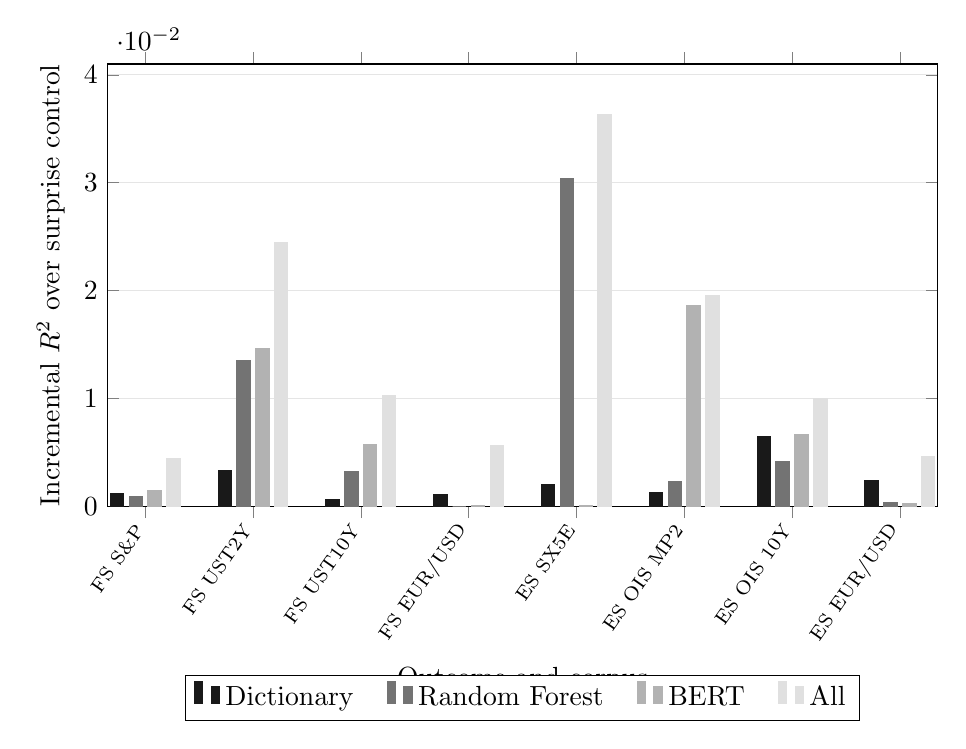
\begin{tikzpicture}
  \begin{axis}[
    ybar,
    width=\textwidth,
    height=7.2cm,
    bar width=4.8pt,
    ymin=0, ymax=0.041,
    xtick={1,2,3,4,5,6,7,8},
    xticklabels={FS S\&P,FS UST2Y,FS UST10Y,FS EUR/USD,ES SX5E,ES OIS MP2,ES OIS 10Y,ES EUR/USD},
    x tick label style={rotate=55, anchor=east, font=\scriptsize},
    ylabel={Incremental $R^2$ over surprise control},
    xlabel={Outcome and corpus},
    legend style={at={(0.5,-0.38)}, anchor=north, legend columns=4, /tikz/every even column/.append style={column sep=0.35cm}},
    ymajorgrids=true,
    grid style={gray!20},
    enlarge x limits=0.05
  ]
\addplot+[fill=DictColor, draw=DictColor]
    coordinates {(1,0.0012) (2,0.0033) (3,0.0006) (4,0.0011) (5,0.0020) (6,0.0013) (7,0.0065) (8,0.0024)};
\addlegendentry{Dictionary}
\addplot+[fill=RFColor, draw=RFColor]
    coordinates {(1,0.0009) (2,0.0135) (3,0.0032) (4,0.0000) (5,0.0304) (6,0.0023) (7,0.0042) (8,0.0004)};
\addlegendentry{Random Forest}
\addplot+[fill=BERTColor, draw=BERTColor]
    coordinates {(1,0.0015) (2,0.0146) (3,0.0057) (4,0.0001) (5,0.0001) (6,0.0186) (7,0.0067) (8,0.0003)};
\addlegendentry{BERT}
\addplot+[fill=AllColor, draw=AllColor]
    coordinates {(1,0.0044) (2,0.0245) (3,0.0103) (4,0.0056) (5,0.0363) (6,0.0195) (7,0.0100) (8,0.0046)};
\addlegendentry{All}
  \end{axis}
  \end{tikzpicture}
  \caption[RQ1 incremental explanatory power chart]{Incremental explanatory
    power of text scores over the rate-surprise control. Bars report the
    increase in $R^2$ relative to an MP1/OIS\_MP1-only model on the common
    sample. Abbreviations: FS = FOMC statements; ES = ECB statements.}
  \label{fig:rq1_method_r2_v31}
\end{figure}

The incremental contribution of text is small for many outcomes and
concentrated in a few cases. For FOMC statements, the strongest incremental
evidence is for the two-year Treasury yield. The rate-surprise-only model
already explains 0.237 of the common-sample variation in UST 2Y reactions.
Adding the Random Forest score raises $R^2$ by 0.014, adding BERT raises
it by 0.015, and adding all three scores raises it by 0.024. The
corresponding coefficient evidence in
Appendix~\ref{app:a2_rq1_coefficients} shows positive and statistically
significant single-score coefficients for RF ($\hat{\beta}=0.017$, $p=0.030$)
and BERT ($\hat{\beta}=0.038$, $p=0.020$). In the joint horse race, the
BERT coefficient remains marginally significant ($p=0.067$), while
dictionary and RF do not independently survive. This is partly attributable to
collinearity: the pairwise correlation between the dictionary and BERT is
0.81 in FOMC statements (Appendix~\ref{app:a3_bert_diagnostics}), producing
variance inflation factors around 3.0 for these two variables. While below the
conventional concern threshold of 5--10, this collinearity means that
individual coefficient significance in the horse race is unreliable, and the
$R^2$ comparison across single-score models is the more informative diagnostic.

\Cref{fig:quintile_ust2y} provides a nonparametric view of the same
relationship. Sorting FOMC statements into quintiles by tone score and
plotting the median UST 2Y reaction shows that the BERT score produces
a nearly monotonic pattern: the most hawkish quintile is associated with
a 1.4 basis point median yield increase, while the most dovish quintile
is associated with a 0.5 basis point decrease. The RF sort shows the
correct direction at the extremes but is noisier in the interior
quintiles, consistent with the RF score capturing decision-predictive
language that does not map cleanly onto a monotonic yield response.

% ══════════════════════════════════════════════════════════════════════════════
% FIGURE — Quintile sort: tone score -> median UST 2Y reaction
% Place in Chapter 6, Section 6.4 (RQ1), after the incremental R² discussion
% and before the press-conference subsection.
% ══════════════════════════════════════════════════════════════════════════════

\begin{figure}[htbp]
  \centering
  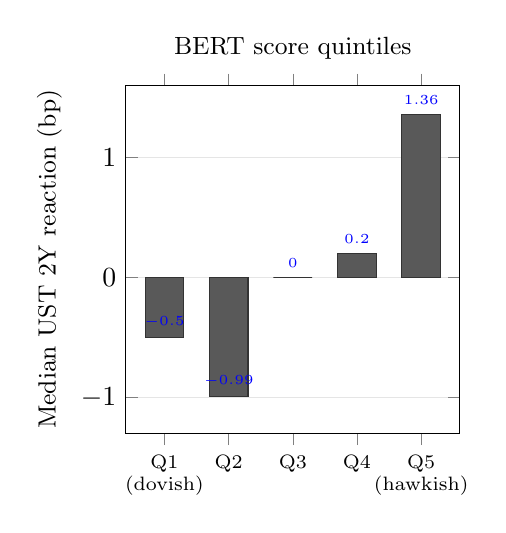
\begin{tikzpicture}
  \begin{axis}[
    ybar,
    width=0.48\textwidth,
    height=6.0cm,
    bar width=14pt,
    ymin=-1.3, ymax=1.6,
    xtick={1,2,3,4,5},
    xticklabels={Q1\\(dovish),Q2,Q3,Q4,Q5\\(hawkish)},
    x tick label style={align=center, font=\scriptsize},
    ylabel={Median UST 2Y reaction (bp)},
    ylabel style={font=\small},
    title={\small BERT score quintiles},
    ymajorgrids=true,
    grid style={gray!20},
    enlarge x limits=0.15,
    nodes near coords,
    nodes near coords style={font=\tiny, /pgf/number format/fixed, /pgf/number format/precision=2},
    every node near coord/.append style={above},
  ]
  \addplot+[fill=black!65, draw=black!80] coordinates {
    (1,-0.50)
    (2,-0.99)
    (3, 0.00)
    (4, 0.20)
    (5, 1.36)
  };
  \end{axis}
  \end{tikzpicture}%
  \hfill
  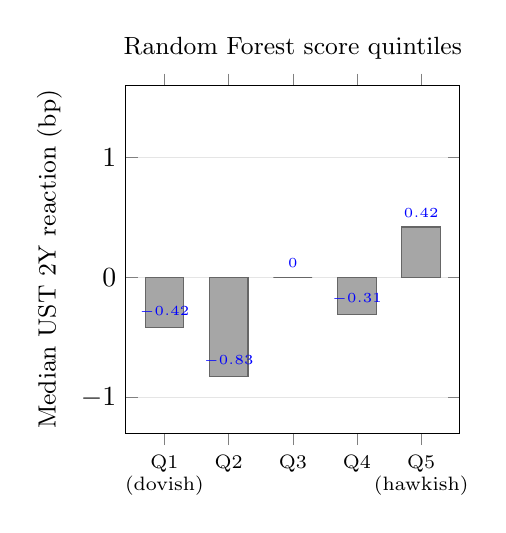
\begin{tikzpicture}
  \begin{axis}[
    ybar,
    width=0.48\textwidth,
    height=6.0cm,
    bar width=14pt,
    ymin=-1.3, ymax=1.6,
    xtick={1,2,3,4,5},
    xticklabels={Q1\\(dovish),Q2,Q3,Q4,Q5\\(hawkish)},
    x tick label style={align=center, font=\scriptsize},
    ylabel={Median UST 2Y reaction (bp)},
    ylabel style={font=\small},
    title={\small Random Forest score quintiles},
    ymajorgrids=true,
    grid style={gray!20},
    enlarge x limits=0.15,
    nodes near coords,
    nodes near coords style={font=\tiny, /pgf/number format/fixed, /pgf/number format/precision=2},
    every node near coord/.append style={above},
  ]
  \addplot+[fill=black!35, draw=black!60] coordinates {
    (1,-0.42)
    (2,-0.83)
    (3, 0.00)
    (4,-0.31)
    (5, 0.42)
  };
  \end{axis}
  \end{tikzpicture}
  \caption[Median UST 2Y reaction by tone-score quintile]{Median
    announcement-window UST 2Y yield change (basis points) by tone-score
    quintile for FOMC statements. Documents are sorted into five equal-sized
    groups by their BERT score (left) or Random Forest score (right), from
    most dovish (Q1) to most hawkish (Q5). A monotonic pattern indicates that
    more hawkish communication is associated with larger yield increases. The
    BERT quintile sort is nearly monotonic; the RF sort shows the correct
    direction at the extremes but is noisier in the interior. $N=237$ for
    BERT; $N=235$ for RF. The relationship is unconditional and does not
    control for the contemporaneous rate surprise.}
  \label{fig:quintile_ust2y}
\end{figure}

\textbf{one pargraph and figure above added by KMC 
}
For FOMC equities and foreign exchange, the text contribution is close to zero.
The incremental $R^2$ values for S\&P 500 and EUR/USD are below 0.006 even in
the full model. This weak evidence is consistent with offsetting channels: a
hawkish statement can raise discount rates, which is negative for equities, but
it can also signal stronger economic conditions, which is positive. Exchange-
rate reactions are similarly difficult to summarise with a single tone
coefficient, because the sign depends on whether markets interpret language
primarily as rate-path news or as information about economic conditions.

For ECB statements, the clearest market result is SX5E. The
rate-surprise-only model explains 0.178 of the common-sample variation. Adding
the RF score raises $R^2$ by 0.030 and the full model raises it by 0.036. The
RF coefficient is positive and statistically significant in the baseline
controlled regression ($\hat{\beta}=0.3713$, $p=0.028$) and remains significant
in the joint horse race ($p=0.045$). The positive sign is consistent with an
information-effect interpretation \citep{nakamura2018,jarocinski2020}: language
associated with tighter policy decisions may also signal stronger macroeconomic
conditions. However, the present design does not structurally separate
monetary-policy news from central-bank information news, so this interpretation
should be read as suggestive rather than as identified evidence of an
information shock. The result also becomes marginal ($p=0.102$) when chair and
era fixed effects are added (Section~\ref{sec:res_fe_fwd_new}), suggesting
that part of the association may reflect cross-president variation rather than
within-regime communication effects.

For OIS\_MP2, BERT provides the largest single-score incremental $R^2$
gain (0.019), but the coefficient is only marginal in the single-score model
and does not survive the full horse race at conventional levels. The evidence
for ten-year yields is weak. The ECB OIS 10Y and EUR/USD regressions have
total $R^2$ below 0.02 in all specifications. FOMC ten-year Treasury reactions
show slightly larger incremental $R^2$ under BERT than under the dictionary,
but the score coefficient is not significant at the 10\% level in the baseline
single-score model. This maturity pattern is intuitive: textual policy tone
should primarily affect short and intermediate maturities, where expected
near-term policy rates dominate, while ten-year rates also embed term premia,
long-run inflation expectations, and global risk factors.


\subsection{Press Conference Evidence}
\label{sec:res_pc_new}

Press conferences extend the RQ1 analysis to a richer communication channel
that includes longer explanations and answers to questions. The evidence is
stronger in some press conference regressions but also less clean because the
FOMC press conference sample is short ($N=91$, starting only in 2011).
\Cref{tab:pc_coefficients_v31} reports the press-conference coefficients
discussed below, so the main text does not rely only on prose-reported
estimates.

\begin{table}[H]
\centering
\caption{Press-conference market-reaction coefficients}
\label{tab:pc_coefficients_v31}
\resizebox{\textwidth}{!}{%
\begin{tabular}{@{}llrrrrrrr@{}}
\toprule
Corpus & Outcome & Dict. & RF & BERT & Dict (joint) & RF (joint) & BERT (joint) & $N$ \\
\midrule
FOMC PC & EUR/USD & 0.191 (0.120) & 0.202\sym{**} (0.090) & 0.457\sym{*} (0.244) & 0.064 (0.137) & 0.160\sym{*} (0.087) & 0.150 (0.275) & 91 \\
FOMC PC & UST 2Y & $-$0.021 (0.020) & $-$0.040\sym{***} (0.013) & $-$0.065\sym{*} (0.035) & 0.007 (0.024) & $-$0.039\sym{***} (0.012) & $-$0.027 (0.045) & 91 \\
FOMC PC & UST 10Y & 0.001 (0.018) & $-$0.020\sym{**} (0.009) & $-$0.051\sym{*} (0.028) & 0.032 (0.030) & $-$0.021\sym{**} (0.008) & $-$0.076 (0.060) & 91 \\
ECB PC & SX5E & 0.174 (0.114) & 0.191 (0.124) & 0.455\sym{**} (0.188) & 0.021 (0.130) & 0.097 (0.135) & 0.389\sym{*} (0.211) & 231 \\
ECB PC & EUR/USD & 0.012 (0.077) & $-$0.159\sym{*} (0.082) & $-$0.035 (0.135) & 0.097 (0.088) & $-$0.187\sym{**} (0.087) & $-$0.030 (0.163) & 231 \\
ECB PC & OIS\_MP2 & $-$0.719 (0.782) & 0.596 (0.943) & 1.772 (1.322) & $-$1.640\sym{*} (0.910) & 0.434 (1.099) & 3.412\sym{**} (1.396) & 224 \\
\bottomrule
\end{tabular}%
}\\[4pt]
\begin{minipage}{\textwidth}
\footnotesize
\emph{Notes}: Entries are coefficients on the text score with HC1 standard
errors in parentheses. Single-score models include the relevant rate-surprise
control. Joint columns report the coefficients from the model containing
dictionary, Random Forest, and BERT scores plus the same control.
\sym{***}, \sym{**}, and \sym{*} denote significance at 1\%, 5\%, and 10\%.
\end{minipage}
\end{table}

For FOMC press conferences, the Random Forest score is significantly
associated with EUR/USD, the two-year Treasury yield, and the ten-year
Treasury yield. The RF coefficient is 0.202 for EUR/USD ($p=0.025$),
$-0.040$ for UST 2Y ($p=0.003$), and $-0.020$ for UST 10Y ($p=0.036$).
These results are robust to Newey-West standard errors with two lags
(the UST 2Y $p$-value remains 0.006; the UST 10Y $p$-value is 0.059),
confirming that the findings are not driven by residual serial correlation.
The results are also not driven by influential outliers: removing the two
meetings with the highest Cook's distance (March 2020 and November 2022)
strengthens the UST 2Y coefficient from $-0.040$ to $-0.049$ ($p<0.001$).

The negative yield signs deserve explicit discussion. The methodology chapter
predicts $\beta>0$ for yields under both the standard monetary-policy channel
and the information effect, yet the FOMC press conference coefficients are
uniformly negative. This is not consistent with a simple ``hawkish language
raises yields'' interpretation. A plausible explanation is that post-2011 press
conferences often combine discussion of tightening conditions with
risk-management or forward-guidance reassurance, so the RF score captures
broader decision-predictive language rather than a clean hawkish yield shock.
The negative sign should therefore be read as evidence that the mapping from
text to yields is more complex than the simple theoretical prediction, rather
than as a robust structural relationship. The positive EUR/USD coefficient is
also unexpected under the standard monetary-policy channel, where hawkish FOMC
language should appreciate the dollar. Like the negative yield signs, it may
reflect the mixed signalling environment of the post-2011 press conference era.

BERT is marginally significant for FOMC press conference EUR/USD and
yields, but these effects weaken in the joint horse race.

For ECB press conferences, BERT is the clearest equity signal. The
coefficient on \bertscore{} in the SX5E regression is 0.455 with $p=0.015$.
The Random Forest score is marginally associated with EUR/USD in the
single-score model ($\hat{\beta}=-0.159$, $p=0.052$) and significant in the
horse race ($p=0.031$). BERT also contributes to the OIS\_MP2 horse
race, where its coefficient is positive and significant ($p=0.015$), though
the large magnitude ($\hat{\beta}=3.41$) and the fact that it is significant
only in the joint model suggest this result should be interpreted cautiously.

\subsection{Dual-Mandate Decomposition}
\label{sec:res_dual_mandate_new}

\Cref{tab:dual_mandate_r2_v31} compares the aggregate dictionary score with
two decompositions. Spec~A uses the aggregate \netscore{}. Spec~B separates
policy-action language from the combined economic score. Spec~C separates
policy, inflation, employment, and residual-risk components. The comparison is
based on the same controlled regression structure as the main RQ1 analysis.
\Cref{fig:dual_mandate_r2_gains_v31} plots the $R^2$ gain from the aggregate
to the full decomposition.


\begin{table}[H]
\centering
\caption{Incremental explanatory power from decomposing dictionary tone}
\label{tab:dual_mandate_r2_v31}
\begin{threeparttable}
\footnotesize
\setlength{\tabcolsep}{5pt}
\renewcommand{\arraystretch}{1.08}
\begin{tabular*}{\textwidth}{@{\extracolsep{\fill}}llrrrr@{}}
\toprule
Corpus & Outcome & $N$ & Spec A & Spec B & Spec C \\
       &         &     & net & policy+econ & full \\
\midrule
FOMC stmt. & S\&P 500 & 232 & 0.0509 & 0.0508 & 0.0562 \\
FOMC stmt. & EUR/USD & 230 & 0.0612 & 0.0607 & 0.0733 \\
FOMC stmt. & UST 2Y & 242 & 0.1912 & 0.1930 & 0.2040 \\
FOMC stmt. & UST 10Y & 242 & 0.0219 & 0.0237 & 0.0316 \\
ECB stmt. & SX5E & 253 & 0.1782 & 0.1842 & 0.1986 \\
ECB stmt. & EUR/USD & 253 & 0.0044 & 0.0046 & 0.0129 \\
ECB stmt. & OIS\_MP2 & 244 & 0.2103 & 0.2192 & 0.2804 \\
ECB stmt. & OIS 10Y & 113 & 0.0158 & 0.0261 & 0.0968 \\
\bottomrule
\end{tabular*}
\begin{tablenotes}[flushleft]
\footnotesize
\item Notes: Spec A uses the aggregate \netscore{}. Spec B separates policy-action language from aggregate economic language. Spec C separates policy, inflation, employment/growth, and residual-risk language. All specifications include MP1 for FOMC outcomes and OIS\_MP1 for ECB outcomes.
\end{tablenotes}
\end{threeparttable}
\end{table}

\begin{figure}[H]
  \centering
  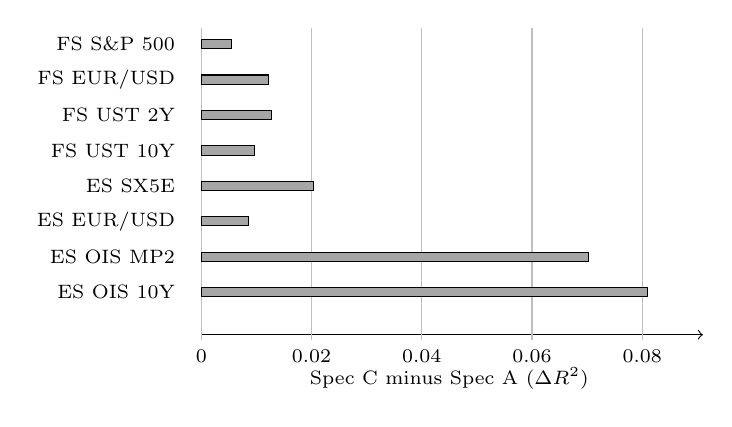
\begin{tikzpicture}[x=70cm,y=0.45cm]
    \draw[->, thin] (0,-9.2) -- (0.091,-9.2);
    \foreach \x/\lab in {0/0,0.02/0.02,0.04/0.04,0.06/0.06,0.08/0.08} {
      \draw[thin, black!25] (\x,-0.55) -- (\x,-9.35);
      \node[anchor=north, font=\scriptsize] at (\x,-9.35) {\lab};
    }
    \foreach \lab/\val/\row in {
      {FS S\&P 500}/0.0054/1,
      {FS EUR/USD}/0.0122/2,
      {FS UST 2Y}/0.0128/3,
      {FS UST 10Y}/0.0097/4,
      {ES SX5E}/0.0204/5,
      {ES EUR/USD}/0.0086/6,
      {ES OIS MP2}/0.0702/7,
      {ES OIS 10Y}/0.0809/8
    }{
      \node[anchor=east, font=\scriptsize] at (-0.003,-\row) {\lab};
      \draw[fill=black!35, draw=black] (0,-\row-0.13) rectangle (\val,-\row+0.13);
    }
    \node[anchor=north, font=\scriptsize] at (0.045,-9.85)
      {Spec C minus Spec A ($\Delta R^2$)};
  \end{tikzpicture}
  \caption[$R^2$ gains from decomposing dictionary tone]{$R^2$ gain from
    replacing the aggregate dictionary score with the full policy, inflation,
    employment/growth, and residual-risk decomposition. Bars report Spec C
    minus Spec A from \Cref{tab:dual_mandate_r2_v31}. FS denotes FOMC
    statements; ES denotes ECB statements.}
  \label{fig:dual_mandate_r2_gains_v31}
\end{figure}


The decomposition is most valuable for ECB yield outcomes. The gain is 7.02
percentage points for OIS\_MP2 and 8.09 percentage points for OIS 10Y,
compared with gains below 1.3 percentage points for all FOMC outcomes. For
FOMC statements, the modest gains are consistent with the FOMC's balanced
communication style, in which policy-action, inflation, and employment
language typically move in the same direction, limiting the benefit of
disaggregation.

For ECB statements, the decomposition is more consequential. For OIS 10Y,
the gain from Spec~A to Spec~C is statistically significant in a partial
$F$-test ($F(3,107)=3.20$, $p=0.027$), and the adjusted $R^2$ rises from
$-0.002$ under Spec~A to $0.055$ under Spec~C: the decomposition turns a
model that explains nothing after degrees-of-freedom correction into one with
modest but genuine explanatory power. The ECB equity gain is smaller but still
visible, rising from 0.178 to 0.199. This result does not mean that the ECB
has a dual mandate in the FOMC sense. Rather, it means that the market
response to ECB communication is component-specific: policy-action language,
inflation language, growth language, and risk language have different
implications for asset prices. Aggregating them into a single net
hawkish--dovish score therefore hides useful variation.

\subsection{Fixed Effects and Forward-Looking Language}
\label{sec:res_fe_fwd_new}

The fixed-effect and forward/current regressions serve as robustness and
decomposition tests for the RQ1 findings reported above. The fixed-effect
ladder supports the main interpretation. The strongest statement-level Random
Forest result, FOMC UST 2Y, is stable across the base model, chair fixed
effects, and chair-plus-era fixed effects. The coefficient is 0.0166 in the
base specification, 0.0175 with chair fixed effects, and 0.0176 with both
chair and era fixed effects; all three estimates are significant at the 5\%
level. The ECB SX5E Random Forest result is stable in magnitude---the
coefficient increases from 0.3713 in the base specification to 0.4094 with
chair fixed effects and 0.4228 with chair and era fixed effects---but the
$p$-value rises from 0.029 to 0.102 in the most saturated specification. This
loss of significance reflects the confounding between ECB president tenure and
rate regime: with only three presidents in the sample (Trichet, Draghi,
Lagarde), chair fixed effects absorb a large share of variation while the
standard error nearly doubles. The baseline $p=0.029$ is the more optimistic
reading and the FE $p=0.102$ is the more conservative one.

\Cref{tab:fe_forward_current_selected_v31} reports the coefficients for
selected forward/current specifications discussed below.

\begin{table}[H]
\centering
\caption{Selected forward/current robustness results}
\label{tab:fe_forward_current_selected_v31}
\begin{threeparttable}
\scriptsize
\setlength{\tabcolsep}{3pt}
\renewcommand{\arraystretch}{1.12}
\begin{tabularx}{\textwidth}{@{}p{2.55cm}c>{\raggedleft\arraybackslash}p{1.85cm}>{\raggedleft\arraybackslash}p{1.85cm}rrX@{}}
\toprule
Corpus/outcome & FE & Forward score & Current score & $N$ & $R^2$ & Interpretation \\
\midrule
FOMC PC, UST 2Y
  & C & $-0.063\sym{*}$ (0.037) & $0.026$ (0.033) & 91 & 0.080
  & Forward tone negative; marginal evidence. \\
FOMC PC, UST 10Y
  & C & $-0.075\sym{**}$ (0.032) & $0.066$ (0.042) & 91 & 0.115
  & Forward tone negative; robust across specifications. \\
ECB statements, SX5E
  & A & $-0.478\sym{**}$ (0.235) & $0.806\sym{**}$ (0.376) & 253 & 0.210
  & Opposite-sign forward/current channel. \\
ECB statements, SX5E
  & C & $-0.456\sym{**}$ (0.225) & $0.833\sym{**}$ (0.375) & 253 & 0.234
  & Stable after chair and broad-era fixed effects. \\
\bottomrule
\end{tabularx}
\begin{tablenotes}[flushleft]
\footnotesize
\item Notes: Entries are coefficients on \netscore{}$^{\text{fwd}}$ and
\netscore{}$^{\text{curr}}$, with HC1 robust standard errors in parentheses.
FE A is the controlled specification without fixed effects; FE C adds
chair/president and broad-era fixed effects. The broader fixed-effect ladder is
reported in Appendix~\ref{app:a2_fe_ladder}. $^{***}$, $^{**}$, and $^{*}$
denote significance at 1\%, 5\%, and 10\%.
\end{tablenotes}
\end{threeparttable}
\end{table}

The forward/backward decomposition is more mixed. In FOMC statements, the
forward-looking dictionary score is negatively associated with S\&P 500
returns in the base specification, but the result disappears after chair and
era fixed effects are added. In FOMC press conferences, forward-looking
dictionary tone is negatively associated with Treasury yields: the UST 10Y
coefficient is approximately $-0.073$ to $-0.075$ across the three
fixed-effect specifications and remains significant at the 5\% level. This is
the clearest evidence that forward-looking language in press conferences
contains information not captured by the aggregate score, although the sign
again points toward a risk-management interpretation rather than a simple
tightening channel.

For ECB statements, the forward/current split is strongest in equities.
Forward-looking tone has a negative coefficient in the SX5E regression, while
current-condition tone has a positive coefficient. Both effects are
significant in the base specification and remain economically similar with
fixed effects. This sign reversal is consistent with forward-looking hawkish
language being interpreted as future tightening (negative for equities) while
current-condition hawkish language is interpreted as evidence of stronger
economic conditions (positive for equities). The pattern provides partial
evidence for the dual-channel interpretation, though it falls short of a
formal structural identification.

\subsection{Additional market outcomes}
\label{sec:res_additional_outcomes}

The broader asset-class screen extends the RQ1 analysis to a wider set of
outcomes, providing evidence that the main conclusions are not artefacts of
selective reporting. Appendix~\ref{app:a2_broad_outcomes} reports controlled
single-score regressions for DXY, TIPS breakevens, additional Treasury
maturities, Euro Stoxx Banks, German Bund yields, and the Italian--German
spread. These additional outcomes do not produce a uniformly stronger pattern
than the headline results. For the FOMC, the clearest additional evidence is
still concentrated around the Treasury curve: RF and BERT scores are positive
for the two- and five-year yields, while thirty-year yields and inflation
breakevens are weak. For the ECB, Euro Stoxx Banks and some sovereign-spread or
Bund-yield regressions show isolated associations, but the signs and significance
are not stable enough to change the main interpretation.

The additional-outcome evidence is therefore useful mainly as a boundary result.
Central bank text is not a universal market-moving variable. It is most
informative for outcomes close to the policy object itself---short and
intermediate yields, medium-term OIS repricing, selected equity reactions, and
future rate decisions. The weaker results for long yields, inflation breakevens,
and sovereign-spread variables are consistent with these assets being more
exposed to term premia, risk premia, fiscal risk, and non-monetary news within
or between announcement windows.

\section{RQ2: Expanding-Window Forecasting Results}
\label{sec:res_rq2_new}

RQ2 evaluates whether central bank language helps predict near-term policy
outcomes and two-year yield changes. The Random Forest forecasting exercise is
the strictest test in the thesis: at each meeting, the model is estimated only
on documents observed before that meeting, and the prediction is made for the
current out-of-sample observation. \Cref{tab:rq2_direct_oos_v31} reports
direct out-of-sample $R^2$ values for the RF forecasts and comparable direct
values for the BERT expanding-window forecasts.
\Cref{fig:rq2_direct_oos_r2_v31} visualises the same contrast.

\begin{table}[H]
\centering
\caption{RQ2 direct expanding-window forecast performance}
\label{tab:rq2_direct_oos_v31}
\begin{threeparttable}
\small
\resizebox{\textwidth}{!}{%
\begin{tabular}{llrrrr}
\toprule
Method & Corpus & \texttt{bps\_next} & \texttt{bps\_next2} & \texttt{y2\_next} & \texttt{y2\_next2} \\
\midrule
RF & FOMC statements & 0.304 & 0.174 & -0.326 & -0.205 \\
RF & FOMC press conferences & 0.237 & 0.148 & -0.207 & -0.132 \\
RF & ECB statements & 0.114 & 0.083 & -0.091 & -0.148 \\
RF & ECB press conferences & 0.054 & 0.014 & -0.172 & -0.023 \\
\addlinespace
BERT & FOMC statements & 0.457 & 0.298 & -0.079 & -0.044 \\
BERT & FOMC press conferences & 0.298 & 0.188 & -0.035 & -0.095 \\
BERT & ECB statements & 0.226 & 0.208 & -0.022 & -0.024 \\
BERT & ECB press conferences & 0.281 & 0.226 & -0.005 & -0.100 \\
\bottomrule
\end{tabular}
}
\begin{tablenotes}
\footnotesize
\item Notes: Entries are direct out-of-sample $R^2$ values from expanding-window predictions. The RF rows are from the Lasso+RF forecast grids. BERT rows are computed from the expanding-window BERT prediction columns in the final corpus files. Negative values mean the forecast performs worse than the sample-mean benchmark. The number of evaluated forecasts ranges from 53 (FOMC PC RF, \texttt{bps\_next}) to 245 (ECB statements); see Appendix~\ref{app:a3_xw_forecasts} for exact counts.
\end{tablenotes}
\end{threeparttable}
\end{table}

\begin{figure}[H]
  \centering
  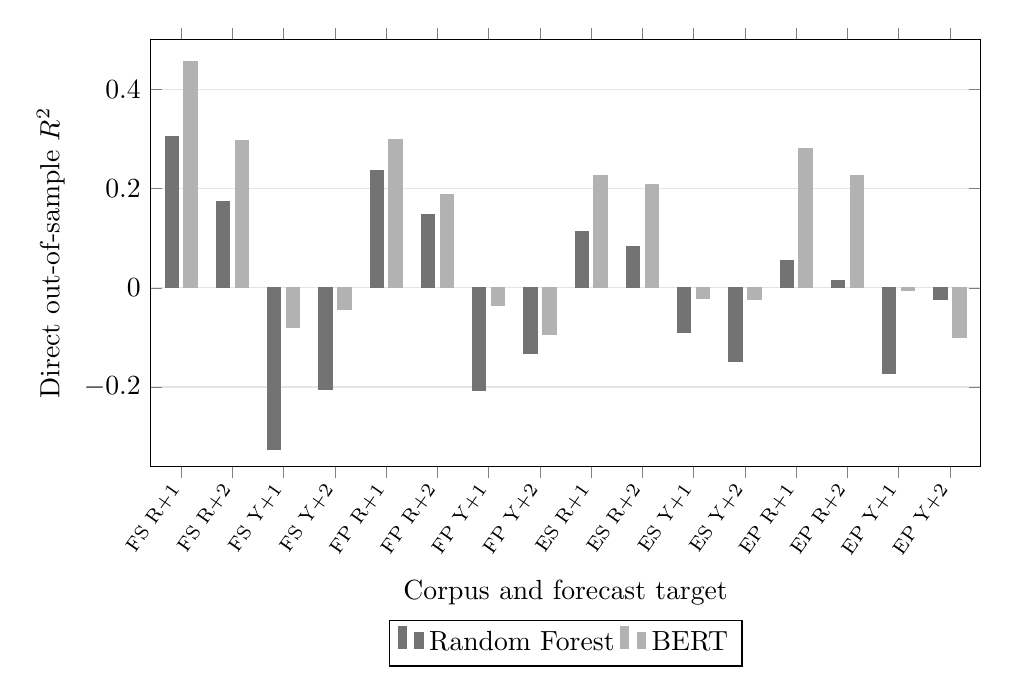
\begin{tikzpicture}
  \begin{axis}[
    ybar,
    width=\textwidth,
    height=7.0cm,
    bar width=4.8pt,
    ymin=-0.36, ymax=0.50,
    xtick={1,2,3,4,5,6,7,8,9,10,11,12,13,14,15,16},
    xticklabels={FS R+1,FS R+2,FS Y+1,FS Y+2,FP R+1,FP R+2,FP Y+1,FP Y+2,ES R+1,ES R+2,ES Y+1,ES Y+2,EP R+1,EP R+2,EP Y+1,EP Y+2},
    x tick label style={rotate=55, anchor=east, font=\scriptsize},
    ylabel={Direct out-of-sample $R^2$},
    xlabel={Corpus and forecast target},
    legend style={at={(0.5,-0.36)}, anchor=north, legend columns=2},
    ymajorgrids=true,
    grid style={gray!20},
    enlarge x limits=0.04
  ]
\addplot+[fill=RFColor, draw=RFColor]
    coordinates {(1,0.3040) (2,0.1740) (3,-0.3260) (4,-0.2050) (5,0.2370) (6,0.1480) (7,-0.2070) (8,-0.1320) (9,0.1140) (10,0.0830) (11,-0.0910) (12,-0.1480) (13,0.0540) (14,0.0140) (15,-0.1720) (16,-0.0230)};
\addlegendentry{Random Forest}
\addplot+[fill=BERTColor, draw=BERTColor]
    coordinates {(1,0.4568) (2,0.2978) (3,-0.0791) (4,-0.0439) (5,0.2983) (6,0.1885) (7,-0.0349) (8,-0.0949) (9,0.2259) (10,0.2080) (11,-0.0222) (12,-0.0244) (13,0.2813) (14,0.2257) (15,-0.0045) (16,-0.1001)};
\addlegendentry{BERT}
  \end{axis}
  \end{tikzpicture}
  \caption[RQ2 direct expanding-window forecast performance]{Direct
    out-of-sample $R^2$ from the expanding-window forecasts. Positive values
    indicate performance above the sample-mean benchmark; negative values
    indicate underperformance. Abbreviations: FS = FOMC statements; FP = FOMC
    press conferences; ES = ECB statements; EP = ECB press conferences; R =
    rate decision; Y = two-year yield change.}
  \label{fig:rq2_direct_oos_r2_v31}
\end{figure}

The first RQ2 finding is that language contains predictive information for
future policy-rate changes, but it does not deliver useful forecasts of future
two-year yield changes. For RF forecasts, direct out-of-sample $R^2$ is
positive for all eight rate-decision targets (two horizons $\times$ four
corpora). It is largest for FOMC statements, where the model reaches 0.304 for
the next decision and 0.174 for the two-meeting-ahead decision. It is smaller
for the ECB, especially in press conferences, but remains positive. In
contrast, all sixteen yield forecasts (two methods $\times$ four corpora
$\times$ two horizons) have negative direct out-of-sample $R^2$. The RF
therefore captures persistent decision-language patterns but does not translate
them into accurate forecasts of future two-year yield movements.

The BERT forecasts strengthen the rate-decision result. The direct
out-of-sample $R^2$ values are positive for all rate-decision targets and
exceed the RF values in each corpus. For FOMC statements, BERT reaches
0.457 for the next decision and 0.298 for the two-meeting-ahead decision. For
ECB press conferences, the corresponding values are 0.281 and 0.226. However,
BERT also fails to deliver direct forecasts of two-year yield changes.

Because rate decisions are highly persistent and holds are common, the
sample-mean benchmark is not the only relevant comparison. The incremental
regressions in \Cref{tab:rq2_incremental_v31} evaluate whether the text
forecasts add information beyond a simple inertia control.
\Cref{fig:rq2_incremental_r2_v31} visualises the same incremental evidence.

\begin{table}[H]
\centering
\caption{Incremental $R^2$ of text forecasts beyond inertia}
\label{tab:rq2_incremental_v31}
\begin{threeparttable}
\small
\resizebox{\textwidth}{!}{%
\begin{tabular}{llrrrr}
\toprule
Method & Corpus & \texttt{bps\_next} & \texttt{bps\_next2} & \texttt{y2\_next} & \texttt{y2\_next2} \\
\midrule
RF & FOMC statements & 0.044 & 0.013 & 0.028 & 0.013 \\
RF & FOMC press conferences & 0.001 & 0.012 & 0.027 & 0.004 \\
RF & ECB statements & 0.013 & 0.006 & 0.005 & 0.007 \\
RF & ECB press conferences & 0.002 & 0.003 & 0.007 & 0.003 \\
\addlinespace
BERT & FOMC statements & 0.012 & 0.010 & 0.017 & 0.012 \\
BERT & FOMC press conferences & 0.105 & 0.064 & 0.008 & 0.007 \\
BERT & ECB statements & 0.011 & 0.005 & 0.071 & 0.005 \\
BERT & ECB press conferences & 0.049 & 0.028 & 0.078 & 0.039 \\
\bottomrule
\end{tabular}
}
\begin{tablenotes}
\footnotesize
\item Notes: Entries are increases in $R^2$ relative to an inertia-only regression. Rate-decision targets control for \texttt{bps\_curr}. Yield targets control for \texttt{y2\_curr}. Positive yield increments should not be interpreted as evidence of standalone yield forecasting ability, since the direct out-of-sample $R^2$ for yield targets is negative in all cases (\Cref{tab:rq2_direct_oos_v31}).
\end{tablenotes}
\end{threeparttable}
\end{table}


\begin{figure}[H]
  \centering
  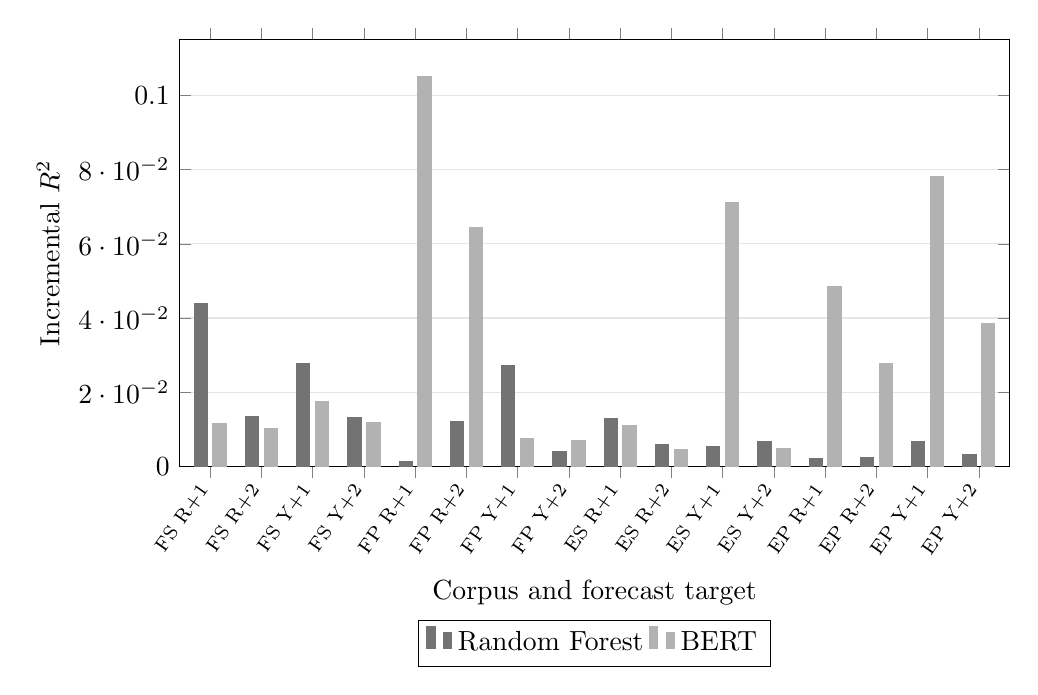
\begin{tikzpicture}
  \begin{axis}[
    ybar,
    width=\textwidth,
    height=7.0cm,
    bar width=4.8pt,
    ymin=0, ymax=0.115,
    xtick={1,2,3,4,5,6,7,8,9,10,11,12,13,14,15,16},
    xticklabels={FS R+1,FS R+2,FS Y+1,FS Y+2,FP R+1,FP R+2,FP Y+1,FP Y+2,ES R+1,ES R+2,ES Y+1,ES Y+2,EP R+1,EP R+2,EP Y+1,EP Y+2},
    x tick label style={rotate=55, anchor=east, font=\scriptsize},
    ylabel={Incremental $R^2$},
    xlabel={Corpus and forecast target},
    legend style={at={(0.5,-0.36)}, anchor=north, legend columns=2},
    ymajorgrids=true,
    grid style={gray!20},
    enlarge x limits=0.04
  ]
\addplot+[fill=RFColor, draw=RFColor]
    coordinates {(1,0.0440) (2,0.0134) (3,0.0277) (4,0.0131) (5,0.0013) (6,0.0121) (7,0.0272) (8,0.0039) (9,0.0128) (10,0.0060) (11,0.0053) (12,0.0068) (13,0.0021) (14,0.0025) (15,0.0068) (16,0.0033)};
\addlegendentry{Random Forest}
\addplot+[fill=BERTColor, draw=BERTColor]
    coordinates {(1,0.0116) (2,0.0103) (3,0.0174) (4,0.0118) (5,0.1052) (6,0.0643) (7,0.0076) (8,0.0069) (9,0.0109) (10,0.0045) (11,0.0710) (12,0.0047) (13,0.0485) (14,0.0277) (15,0.0781) (16,0.0385)};
\addlegendentry{BERT}
  \end{axis}
  \end{tikzpicture}
  \caption[Incremental $R^2$ of text forecasts beyond inertia]{Incremental
    $R^2$ from adding the expanding-window text forecast to an inertia-only
    baseline. Rate-decision targets control for the current rate decision;
    yield targets control for the current two-year yield change. Abbreviations
    follow \Cref{fig:rq2_direct_oos_r2_v31}.}
  \label{fig:rq2_incremental_r2_v31}
\end{figure}

The largest incremental gains come from BERT in press conferences: 10.5
percentage points for the next FOMC decision, 6.4 percentage points for the
two-meeting-ahead FOMC decision, 4.9 percentage points for the next ECB
decision, and 2.8 percentage points for the two-meeting-ahead ECB decision.
The concentration of BERT incremental power in press conferences is consistent
with press conferences containing more explicit forward-looking policy
discussion, which the sentence-level model is designed to capture. The Random
Forest adds its largest incremental rate-decision signal in FOMC statements,
where the gain is 4.4 percentage points for the next decision.

The inertia baseline is substantial for rate decisions. In the FOMC statement
sample, the current decision alone explains 48.2\% of the variation in the
next decision over the RF forecast sample. Adding the RF text forecast raises
this to 52.6\%, an incremental gain of 4.4 percentage points, and the RF
forecast coefficient is statistically significant ($p=0.005$). For ECB
statements, the RF next-decision increment is smaller, 1.3 percentage points,
but the forecast coefficient remains significant ($p=0.043$). In ECB press
conferences, the RF forecast adds almost no incremental rate-decision
information beyond inertia.

The BERT forecast adds the most incremental rate-decision information
in press conferences. For FOMC press conferences, adding the BERT
next-decision forecast raises $R^2$ by 10.5 percentage points relative to the
inertia baseline, and the forecast coefficient is significant at the 1\%
level. For ECB press conferences, the corresponding increment is 4.9
percentage points, also significant at the 1\% level. This suggests that
sentence-level semantic tone is particularly useful in longer explanatory
documents, where central bankers discuss the likely future path of policy more
explicitly than in short statements.

One interpretive caveat applies to the rate-decision forecasts. All three text
scores are highly autocorrelated: the first-order autocorrelation of
\netscore{} is 0.87 for FOMC statements, 0.84 for FOMC press conferences, and
the RF and BERT scores are similarly persistent ($\rho_1 \approx 0.55$--$0.78$
across corpora). Part of the forecast power may therefore reflect the text
score acting as a slow-moving proxy for the policy stance, rather than
capturing meeting-specific forward-guidance signals. The incremental $R^2$
analysis partially addresses this concern by controlling for the current rate
decision, but persistent text scores may still capture slow-moving stance
information not fully absorbed by the single-lag inertia control.

The yield-forecast results warrant a clear negative conclusion. Some
regression-based incremental $R^2$ values are positive, especially for BERT in
ECB yield specifications. However, the direct out-of-sample $R^2$ values are
negative for all sixteen yield targets across both methods and all corpora. The
conclusion is therefore unambiguous: central bank language does not predict
subsequent two-year yield changes out of sample. This distinction is
economically plausible. Future rate decisions are partly governed by central
bank communication and policy inertia, whereas future yield changes also
reflect incoming macroeconomic data, risk premia, market positioning, and
global shocks between meetings.

As an additional interpretability diagnostic, Appendix~\ref{app:rf_single_xw_importance}
reports variable importance from one illustrative expanding-window Random Forest
forecast. This diagnostic is model-level and should not be interpreted as a local
causal explanation of a single prediction.

\section{Synthesis of Results}
\label{sec:res_synthesis_new}

The empirical results support three central conclusions, each subject to the
limitations discussed below.

First, central bank language contains measurable information, but the type of
information depends on the scoring method. The dictionary and BERT
scores agree strongly for statements, especially ECB statements, but diverge
substantially in press conferences. The Random Forest is closest to the
contemporaneous rate-decision benchmark because it is trained on that object.
This is useful for classification but should not be interpreted as independent
evidence that the Random Forest discovers the true economic stance of
communication.

Second, the answer to RQ1 is conditional rather than universal. Textual tone
explains some announcement-window market reactions after controlling for rate
surprises, but the effects are concentrated in specific asset classes and
methods. The strongest statement-level evidence is for FOMC two-year yields
(where RF and BERT coefficients are significant and the result survives
Newey-West standard errors and fixed-effect controls) and ECB equities (where
the RF coefficient is significant in the baseline but marginal with full fixed
effects). Equities and exchange rates do not show a stable dictionary-based
relationship across corpora. Ten-year yield evidence is weak.

Third, the answer to RQ2 is positive for future policy decisions and negative
for future yields. Both RF and BERT produce positive direct expanding-window
$R^2$ values for next-meeting and two-meeting-ahead rate decisions in all eight
corpus--method pairs. The same is not true for two-year yield changes, where
all sixteen direct out-of-sample $R^2$ values are negative. Communication
helps forecast the central bank's own subsequent policy actions, but it does
not forecast the market's subsequent yield adjustment.

\subsection*{Limitations}

Several limitations should be kept in mind when interpreting these results.

\emph{Multiple testing.} The chapter reports results across four corpora,
multiple outcomes, three methods, and several regression variants (horse race,
fixed-effect ladder, forward/current decomposition, dual-mandate
decomposition), generating in excess of 200 individual regression
specifications. No formal multiple-testing correction has been applied. While
individual $p$-values should therefore be interpreted conservatively, the
patterns that are consistent across methods and outcomes---such as the positive
rate-decision forecasting result, which holds for all eight corpus--method
pairs---are less likely to reflect spurious significance than isolated results.

\emph{Residual leakage in the Random Forest.} Approximately 18--20\% of the
Random Forest's feature importance in FOMC and ECB statements is attributable
to terms that correlate with specific speakers or eras rather than with
economic stance. The \rfscore{} used in the RQ1 regressions is therefore
partly influenced by era-specific vocabulary. The dictionary and BERT
scores, which are not trained on the rate decision, provide a cleaner test of
the communication channel.

\emph{BERT domain transfer.} The sentence-level classifier exhibits a
systematic dovish shift, particularly in press conferences, likely reflecting
domain transfer from the FOMC-trained classifier. While the continuous score
retains meaningful variation, the low discriminative power for hawkish
classifications limits the method's usefulness for identifying hawkish
communication events.

\emph{Text score persistence.} All three text scores are highly autocorrelated
($\rho_1 \approx 0.55$--$0.87$ across corpora), which means part of the RQ2
forecasting power may reflect the text score acting as a slow-moving proxy for
the policy stance rather than capturing meeting-specific forward guidance. The
incremental $R^2$ analysis partially addresses this concern by controlling for
the current rate decision, but persistent text scores may still capture
slow-moving stance information not fully absorbed by the single-lag inertia
control.

Overall, the results favour a layered interpretation of central bank
communication. Dictionary scores provide transparent and theoretically
structured measures. Random Forest scores capture decision-predictive language
that is useful for classification and some market-reaction regressions.
BERT scores capture semantic information that is especially useful in
press conferences and in expanding-window rate-decision forecasts. The methods
are therefore complementary, but their economic interpretation differs. The
evidence is most persuasive when the outcome is close to the communication
object itself---the next policy decision or short-maturity yields---and weaker
when the outcome is more exposed to competing macro-financial forces.